\section{Solution strategies}
\label{sec:solution-strategies}

Since not all challenges are likely to be solved in the first place, a primary task would be the focusing on critical issues to at least boosting the project's overall performance noticeably without losing too much track. This may be worked on in terms of collaboration, as well as in the project's setup, where on the one hand the team's performance and on the one hand the build engine's performance should be improved.

Interestingly, a lot of issues could be covered using GitHub's API, although some project specific adaptions are still necessary. Nevertheless, it provides enough information for quickly perceiving a sufficient overview of the respective repository.


\subsection{Distributed development}
\label{sec:solutions-distributeddevelopment}

Based on GitHub's API and the advantages of using Git as version control system, it is definitely a significant benefit to equip all project contributors with a GitHub account. While the public, open-source model is free of charge (see ch. \ref{sec:github-history} on p. \pageref{sec:github-history}), there are also different pricing models offered for privately held projects, which should be hidden to the public, starting at 25\$ per month (including 5 user accounts)\footnote{\url{https://github.com/pricing} -- GitHub's pricing models.}.

Although dependent on financial expenditures, the additional value of working on a project with closed source (though it may be released as open source somewhere in the future) may be worth considering. Yet, full-featured access to the API is also included in the free tier though.

Not only GitHub offers a queryable API, also \emph{Bitbucket} provides REST endpoints with similar response data\footnote{\url{https://developer.atlassian.com/bitbucket/api/2/reference/} -- Bitbucket's API documentation.}, although certain features are missing, compared to GitHub. These missing features include for example certain project download functions, among others.

In addition to the API, the built-in In-Page Code Editor (among others) plays an important role for choosing GitHub as core support tool for this project. Therefore, merging using pull requests and a continuous branching model for supporting staging versions qualify as strategies for proposal to developers.


\subsection{Build cycles}
\label{sec:solutions-remotebuilding}

Supporting content authors in their workflow also means to not require them to install unnecessary build tools manually, unless critically needed. Due to the possibility of using GitHub's In-Page Editor, the whole Git checkout, commit and push process becomes in a way redundant too. Moreover, the online editor automatically creates pull requests on demand, so that the respective project owners should get notified automatically, if a merge is possible and therefore an update of the currently published project may be initiated.

Normally, a responsible user would pull the new state after a merge of the pull request, then execute the build pipeline. After the build process succeeded, he/she then has to take care for updating the webroot on the server, so that the newest version of the website gets delivered to the client upon request. However, this practice may easily get cumbersome, as the respective developer might get distracted by checking out new branches and possibly leaving behind his/her own work for the moment. Moreover, if the deployment has to be done manually, additional mistakes may happen during the whole action.

In this case, it makes sense to remotely outsource the build service and to possibly even automatically execute the render cycle. Used in conjunction with GitHub's \emph{Webhooks}, an external service would receive a build execution order via a HTTP POST request, based on certain predefined events in the GitHub repository \cite{GithubWebhooks}. Apart from the information the webhook provides, the service would even accept custom build options issued by responsible users, as the endpoint has to be publicly available anyhow. Once a build succeeds, the service should then notify a predefined list of users about the render cycle result and provide the outcome via download possibility.

\subsubsection{Existing remote services}
\emph{CloudCannon}\footnote{\url{http://cloudcannon.com} -- CloudCannon, the Cloud CMS for Jekyll.} is probably the most popular online static site generator and offers an external building service for Jekyll projects, together with source access using a GitHub or Bitbucket repository. The service is commercial, starting at 25\$ per month and user\footnote{\url{http://cloudcannon.com/pricing/} -- CloudCannon's pricing page.}. According to its documentation, it supports Jekyll projects running v2.4.0 or newer\footnote{\url{https://docs.cloudcannon.com/building/versions/} -- Supported versions on CloudCannon documentation.}. It features a project file explorer and presents every new project as opinionated as Jekyll usually does (see ch. \ref{ec:jekyll-technology} on p. \pageref{ec:jekyll-technology}), as well as an automatic deployment service on their own subdomains. However, access to the built distribution files is not included, so that every external deployment needs a full rebuild beforehand.

\paragraph{}
\emph{BowTie}\footnote{\url{https://bowtie.io} -- Website of BowTie.} is similar to CloudCannon, also offers a commercial CMS service for Jekyll -- plans start at 10\$ per month\footnote{\url{https://bowtie.io/pricing/} -- BowTie's pricing page.}. It seems to be a much more standalone service than CloudCannon, though it also offers GitHub integration, as well as custom Webhooks for event-based actions on external services.

\paragraph{}

%% Screenshot of Pancake push fail
\begin{figure} % h-ere, t-op, b-ottom, p-age
    \centering
    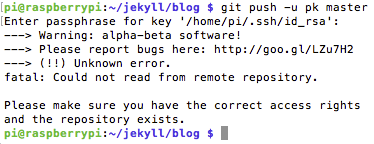
\includegraphics[width=0.75\textwidth]{remote-pancake.png}
    \caption{A screenshot of trying to push a Jekyll project to \emph{Pancake}. The operation failed with an ``Unknown error'' and a message, stating ``Warning: alpha-beta software!''.}
    \label{fig:remote-pancake}
\end{figure}
%
\emph{Pancake}\footnote{\url{https://www.pancake.io} -- Website of Pancake.} is a free service for externally building static sites. It features an engine auto-detection and currently supports \emph{Jekyll, Wintersmith, Pelican, Sphinx, Hyde} and \emph{Middleman}\footnote{\url{https://github.com/pancakeio/detect/blob/master/heuristics.go} -- Currently supported static site generators by Pancake in raw source file on GitHub.}. Due to its non-commercial version, several restrictions are to be considered \cite{PancakeGitProjects}.

However, after trying to push a newly generated Jekyll project to their service via Git, it failed with an \emph{Unknown error}, stating it is still considered ``alpha-beta software'' (see Fig. \ref{fig:remote-pancake}). It seems that Pancake uses a post-receive hook for automatically trying to build a project, once it detected the underlying engine type. This causes waiting time for the developer on the one hand, but on the other hand informs whether a build was successful or failed. During another push attempt, it failed, as \emph{bundler}\footnote{\url{http://bundler.io} -- Bundler, a gem dependency manager.}, a gem dependency management tool required by Jekyll, was not mentioned in the ``Gemfile'' contained in the repository.


\subsection{Caching}
\label{sec:solutions-caching}

As stated before, most static site generators do not contain any form of caching mechanism by default -- if they do, caching is limited to the local machine a build is executed on. Since there is probably not an easy way of providing a form of remote caching, as this largely includes the necessity of external services to exchange a common status, as well as an index containing informations about source and destination files for later rebuilds, it needs an equivalent strategy, which merely contains these informations from a certain point in the past to the present, without relying on physical file structures to be exchanged.

Furthermore, such a caching strategy must be universally useable across all operating systems and ideally does not require any additional setup from the user. Moreover, it should also feature hassle-free integration into any project without depending on an external, yet unused service.

Keeping all of these proposals under consideration, it is possibly certain, that not every suggestion might get featured equally in the final solution -- the main reason is, that a kind of transformation like the one caused by a build pipeline always needs an existing status to build up from. So, tradeoffs are likely to accompany any form of decision to be made in this case.

\subsubsection{Caching by diff}
As Git was chosen as version control system, diff is already part of the development suite. Therefore, a gapless detection of development progress between two arbitrary commits is possible. While diff might not be the most human-friendly syntax, especially when working with huge data sets, it can be parsed to JSON using different third-party tools. Thus, its usability for further processing on application level is assured\footnote{\url{https://runkit.com/saschazar21/diff-parsing-demo} -- An interactive example for fetching and parsing a diff-file.}.

The probably most important parts of a diff representation are the different file paths, as well as the type of modification each affected file was put through in the respective time span. Considering this kind of information, an existing repository might be quickly divided into unaffected and affected files -- thus ending up in the realization, that affected files, as well as their dependents possibly need to be selected for a rebuild. The final decision of the rebuild extent based on the diff, however, is the responsibility of the developer, as it should be merely seen as recommendation than as obligation.

To conclude the consideration of using diff, it might be said, that the approach explained above nearly has not to do anything with ``classical'' caching. The explanation for this statement is simple, as such a mechanism, founded on diff, is not dependent on support-files produced on its own (like a caching catalogue). It merely has to rely on a complete and  successful environment, built with the currently selected \emph{base} commit as its \emph{head}, so that the current diff instance may begin its evaluation from the last successful build state. Its primary flaws are therefore its ``blindness'' towards the completeness of the file tree it has to build up on.
